% !TeX spellcheck = en_US
\documentclass[conference]{IEEEtran}

% *** GRAPHICS RELATED PACKAGES ***
%
\usepackage[pdftex]{graphicx}
% declare the path(s) where your graphic files are
\graphicspath{{./figures/}}
% and their extensions so you won't have to specify these with
% every instance of \includegraphics
\DeclareGraphicsExtensions{.pdf,.jpeg,.png}

% *** MATH PACKAGES ***
%
\usepackage{amsfonts,amsmath,amssymb} % Mathematical symbols.

% correct bad hyphenation here
\usepackage{listings}
\usepackage{cite}
%\usepackage{caption}
\hyphenation{UPPAAL}
\newcommand{\thetatool}{\textsf{theta}}
\newcommand{\Thetatool}{\textsf{Theta}}
\newcommand{\Yakindu}{\textsf{Yakindu}}

\begin{document}

\title{The Composition Language of the \\ Gamma Framework}


% author names and affiliations
% use a multiple column layout for up to three different
% affiliations
\author{\IEEEauthorblockN{Bence Graics, Vince Moln\'ar}
\IEEEauthorblockA{Budapest University of Technology and Economics, \\
Department of Measurement and Information Systems \\
Budapest, Hungary \\
Email: \texttt{bence.graics@gmail.com},  \texttt{molnarv@mit.bme.hu}}

}

% make the title area
\maketitle

% As a general rule, do not put math, special symbols or citations
% in the abstract
\begin{abstract}
%	Many of today's safety-critical systems are reactive, embedded systems. Their internal behavior is usually represented by state-based models. Furthermore, as the tasks carried out by such systems are getting more and more complex, there is a strong need for compositional modeling languages. Such modeling formalisms start from the component-level and use composition to build the system-level model as a collection of simple modules.
%	There are a number of solutions supporting the model-based development of safety-critical embedded systems. One of the popular open-source tools is Yakindu, a statechart editor with a rich language and code generation capabilities. However, Yakindu so far lacks support for compositional modeling.
%	This paper proposes a formal compositional language tailored to the semantics of Yakindu statecharts. We propose precise semantics for the composition to facilitate formal analysis and precise code generation. Based on the formal basis laid out here, we plan to build a complete tool-chain for the design and verification of component-based reactive systems.
\end{abstract}

% no keywords




% For peer review papers, you can put extra information on the cover
% page as needed:
% \ifCLASSOPTIONpeerreview
% \begin{center} \bfseries EDICS Category: 3-BBND \end{center}
% \fi
%
% For peerreview papers, this IEEEtran command inserts a page break and
% creates the second title. It will be ignored for other modes.
\IEEEpeerreviewmaketitle



%\section{Introduction}
%As the complexity of software systems increases, more and more responsibility falls onto system engineers who have to supervise the design, implementation and analysis of interacting system components. Therefore, techniques and tools that support the design and development of correct systems are needed. Such tools and techniques are of high priority in the domain of safety-critical systems.
%
%Proving correctness is an important requirement when designing safety critical systems. In addition to testing, \emph{formal methods} can be applied to verify the correctness of the system design in an early phase. A common approach to state-based behavior analysis is \emph{model checking}. Unfortunately, most of the modeling formalisms developed for engineers are not suitable for direct analysis purposes, therefore formal models usually have to be created manually by an expert team.
%
%To address these problems, we created a framework that supports the design, formal verification, validation and composition of state-based engineering models. These models are based on \Yakindu, which supports the creation of complex hierarchical statecharts with a graphical editor, validation and simulation features. \Yakindu, also supports source code-generation from statecharts to various languages (Java, C, C++) which is reused by our framework.
%
%This work is structured as follows\dots

%\section{Approach}
%
%Designers use engineering models to define the behavior of systems. These modeling languages have a large element set which enables their users to express
%their thoughts and ideas as freely and concisely as possible. On the other hand, the high abstraction level and complexity of such models make it impossible to formally analyze such models which is fundamental in safety-critical system design.
%
%The formal verification of models can be done only in an analysis language. Therefore, a model transformation has to be defined that generate analysis models from engineering models. These formal languages tend to have a small element set which hampers the the definition of such model transformations. This problem is called \emph{abstraction gap}.
%
%
%In our framework we addressed the problem of the abstraction gap by introducing a formal intermediate language called \thetatool. This approach splits the large model transformation process into two smaller ones making them easier and more maintainable.  Additionally, the intermediate language enables the framework to be extended with both engineering and analysis modeling languages.
%
%
%The analysis language supported by our framework is UPPAAL. The formal modeling language of UPPAAL is based on the finite automaton formalism. Furthermore, it supports timing expressions, it is well-documented and freely available for academic use.
%
%During the design of complex systems the created models tend to become unmanageably large which encumbers flaw-correction and maintenance. Many times the resulting model could be decomposed into smaller units that interact with each other, thus implementing the original behavior. Our framework supports the composition of behavioral models based on the \thetatool\ intermediate language and a simple domain specific language (DSL). Presently, the composition of \Yakindu\ statecharts is supported, but the framework is extensible with arbitrary behavioral models as long as they can be transformed to the intermediate language. 

%The intermediate language enables the composition of  models.\footnote{The composition of models of different languages is supported as well, only a transformation has to be defined to the intermediate language.} 

\section{Introduction}

%As the complexity of software systems increases, more and more responsibility falls onto system engineers who have to supervise the design and implementation of interacting system components. Extra effort has to be invested into the analysis of systems in the safety-critical domain. Safety-critical systems are often operated in embedded environments.
%
%Embedded systems are designed for a well-defined, special task. In order to execute this task they interact with their environments. They sense certain parameters of their environments and often have control tasks. This is supported by the use of sensors and actuators. For these reasons, embedded systems are considered reactive system.

Statechart \cite{Harel:1987:SVF:34884.34886} is a widely used formalism to design complex and hierarchical reactive systems. Among the many statechart tools, our work is based on the open-source \Yakindu\footnote{https://itemis.com/en/yakindu/statechart-tools/}, which supports the development of complex hierarchical statecharts with a graphical editor, validation and simulation features. \Yakindu\ also supports source code-generation from statecharts to various languages (Java, C, C++).

The requirements embedded systems have to meet are getting more and more complex. Therefore, the models created for such systems tend to become unmanageably large, which encumbers extensibility and maintenance. Instead, the resulting models could be created by composing smaller units. These units interact with each other using the specified connections, thus implementing the original behavior. There are several tools that aim to support this methodology.

SysML \cite{OMGSysML,Delligatti:2013:SDB:2560076} tools have a large set of modeling elements which enables their users to express their thoughts and ideas as freely and concisely as possible. On the other hand, they rarely define precise semantics, which encumbers code generation and analysis. BIP \cite{Basu:2006:MHR:1158333.1158344,konnov_et_al:LIPIcs:2016:6167,Bozga:2009:MSS:1629335.1629347} is a compositional tool with well-defined semantics that supports the formal verification of modeled systems. Source code generation is also possible with this tool. Scade\footnote{http://www.esterel-technologies.com/products/scade-suite/} \cite{bghm14,venky_08_statemate} is a tool that unifies the advantages of design and analysis tools. It supports the generation of source code as well as the formal verification of the modeled system. It is a commercial tool and does not support extensibility.
Matlab Stateflow \cite{Chen2016} is an environment for modeling and simulating decision logic using statecharts and flow charts. It is a leading tool for composing state-based models in the domain of safety-critical embedded systems. It supports the encapsulation of state-based logics which can be reused throughout different models and diagrams.

Unfortunately, \Yakindu\ does not support composition features. The main goal of our work is to create a tool that enables the users to compose individual statechart components into a single composite system by constructing connections through ports. The ultimate goal of this work is to enable code generation and formal verification of composite models with model transformations based on the proposed semantics.

We will call this type of composition an event-based automata network, as opposed to dataflow networks, which can be considered message-based automata networks in this sense. In event-based automata networks, data is only of secondary importance -- the occurrence of the event is in focus. In message-based settings, data is more significant, thus message queues are desirable to buffer the simultaneous messages.

This paper is structured as follows. Section \ref{sec:yakindu_semantics} presents the semantics of \Yakindu\ statecharts serving as the basis of the compositional language. The syntax and semantics of the compositional language along with an example are introduced in Section \ref{sec:compositional_language}. Finally, Section \ref{sec:conclusion} provides concluding remarks and ideas for future work.

\begin{figure*}[!t]
	\centering
	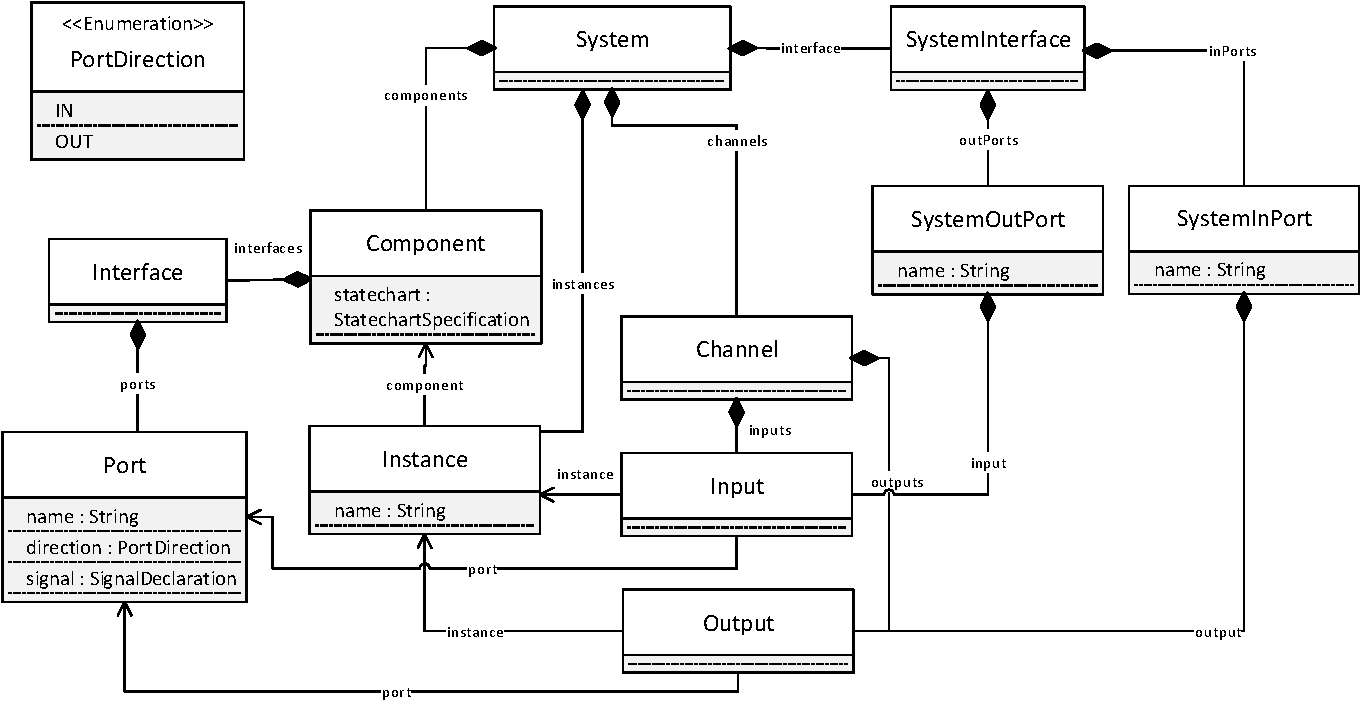
\includegraphics[width=0.85\textwidth]{figures/metamodel_cropped2}%	
	\caption{Metamodel of the compositional language.}
	\label{fig:metamodel}
\end{figure*}

\section{Abstracting Yakindu Statecharts}
\label{sec:yakindu_semantics}
\Yakindu\ adopts a statechart formalism which is the extension of the well-known state machine formalism. Statecharts support the definition of auxiliary variables as well as concurrency and state refinement. This section introduces a syntactical abstraction of \Yakindu, i.e.~the actual model elements are ignored. We deal only with the input and output events in addition to the actual state configuration, but not the semantics. This way we can generalize the composition of abstract models with minimal restrictions to the usable formalisms. In this approach, a \Yakindu\ statechart is considered a 5-tuple: $\mathbb{S} = \langle I, O, S, s_0, T \rangle$ where:
\begin{itemize}
	
	\item $I$ is a finite set of input events (from the environment)
	
	\item $O$ is a finite set of output events (for the environment)
	
%	\item $E = I \cup O$ is the union of input and output events
	
%	\item $V = \{void, boolean, integer, real, string\}$ is the supported parameter types of events
%	
%	\item $W\colon E \rightarrow V$ assigns a type to each event
%	
	%\item $V$ is a finite set of boolean, integer, real and string variables (MI LEGYEN A SOKFÉLE TÍPUSSAL?)
	
	%\item $W\colon V \rightarrow \{0, 1, \cdots\}$ assigns values to the variables (ITT NEM CSAK INTEGER KÉNE)
	
	\item $S = \{s_1, s_2, \cdots , s_n\}$ is a finite set of states, including a state configuration and values of variables
	
	%\item $\Omega \subseteq S \times \{W\}$ is a finite set of statechart states, i.e.~a state configuration and values assigned to the variables
	
	\item $s_0 \in S$ is the initial state	
	
	\item $T \subseteq (2^I \times S) \times (S \times 2^O) $ is a finite set of transitions, that represent changes of state in response to a set of input events and generate a set of output events
\end{itemize}

 \Yakindu\ statecharts adopt a turn-based semantics. 
 The following paragraphs introduce the interpretation of \emph{turns} as well as how the raising of events is associated to them.
 
 Events represent signal receptions. There are two types of events: \emph{simple} or \emph{void} events and \emph{parameterized} or \emph{typed} events. The latter enables the modeling of parameterized signals, which can describe additional details. Note that multiple input events can be raised in a single turn according to the abstract formalism defined above. In \Yakindu\ the raising of events is interpreted as setting a boolean flag to true. \Yakindu\ therefore does not support message queues. Owing to this semantics raising the same \emph{simple} event in a particular turn once or several times has the same effect. On the other hand, \emph{parameterized} events are defined by their parameter as well, so a new event raising with a different parameter overwrites the former one. Although this behavior is an essential part of the semantics of \Yakindu, it is not relevant either in the abstract formalism presented above or the semantics of the composition language defined in Section \ref{sec:semantics}.

 All turns consist of two distinct sections, a \emph{raising} section and a \emph{running} section. In the raising section input events of the statechart are raised as presented in the previous paragraph. This is followed by the running section where a new stable state of the statechart is defined. It starts with the examination of the transitions going out of the particular state configuration. The goal is to specify the firing transition. At this point a \emph{race condition} might exist if multiple outgoing transitions are enabled, e.g.~more of them are triggered by raised input events. \Yakindu\ intends to solve ambiguity by introducing the concept of \emph{transition priority}: users can specify which of the outgoing transitions of a state should be fired in case of a race condition by defining a total ordering of the transitions. The firing transition specifies the next stable state of the statechart, including the state configuration, values of variables and events for the environment.
 
 %In our work we defined statechart validation rules in order to support validation at an early stage of statechart design. We put emphasis on finding possible race conditions, thus prompting the users not to rely on transition priority. Additionally, the rules check unreferred variables and events, transitions occluded by transitions of parent states,  transitions connecting nodes of parallel regions and race conditions in parallel regions. Practically, the goal of these constraints is facilitating the design of well-formed statecharts whose composition and emergent behavior is deterministic and analyzable. 


\section{Language for Composition}
\label{sec:compositional_language}
%The compositional language is based on Xtext\footnote{http://eclipse.org/Xtext/} due to its easy-to-use language and the additional features it provides, e.g.~a parser, a linker, a compiler and content assist.

This section defines the syntax of the compositional language and introduces the semantics the composite system conforms to. This semantics is heavily influenced by the statechart semantics defined by \Yakindu\ and strives to address some of its problems, e.g.~gives the ability to parallel regions to communicate with each other. 

\subsection{Syntax}

Figure \ref{fig:metamodel} depicts the metamodel of the compositional language. The root element in the metamodel is the \textsl{System}. A \textsl{System} contains \textsl{Components} which refer to \Yakindu\ statecharts as well as \textsl{Instances} of such \textsl{Components}. Each \textsl{Component} has an \textsl{Interface} that contains \textsl{Ports}. Through \textsl{Ports}, signals of statecharts can be transmitted or received according to their directions.

\textsl{Channels} can be used for defining the emergent behavior of the composite system. A \textsl{Channel} has one or more \textsl{Inputs} and one or more \textsl{Outputs}. An Input of a \textsl{Channel} connects to an output \textsl{Port} of an \textsl{Instance} and vice versa. Whenever a \textsl{Channel} receives a signal through any of its \textsl{Inputs}, the signal is sent to each \textsl{Output}, i.e.~to the corresponding input \textsl{Ports} of \textsl{Instances}. The language does not support connecting \textsl{Ports} of the same direction and a validation rule is defined that marks incorrect connections.

The language supports the definition of an interface through which the composite system interacts with its environment. This is the \textsl{SystemInterface} that contains \textsl{SystemPorts}. \textsl{SystemPorts} are aliases of \textsl{Ports} of  \textsl{Instances}. If a signal arrives to a \textsl{SystemInPort}, it will be forwarded to the \textsl{Port} of the referred \textsl{Instance} instantly. \textsl{SystemOutPorts} work similarly, but with output \textsl{Ports} of \textsl{Instances}. 
%
%\begin{itemize}
%	
%	\item Components: A Component refers to a \thetatool\  Statechart specification. For each Component an Interface has to be defined.
%	
%	\item Interface: An Interface of a Component is composed of Ports. An Interface does not need to have a Port declaration for each \thetatool\ Signal declaration defined in the Statechart specification. 
%	\item Port: Ports are endpoints the Instances of the particular Component will send or receive signals on. A Port refers to a \thetatool\ Signal declaration and it also has a direction (IN or OUT). A Port with the direction of IN may only \emph{receive} signals, OUT ports are for \emph{transmitting} signals. A Signal declaration referred to by a Port may have a type. This means values can be transmitted through signals. 
%	
%	\item Instances: Instances can be instantiated of Components. A Component may have multiple instantiations or none at all.
%	\item Channels: Connecting Ports of multiple instances can be defined using Channels. A Channel has one or more Inputs and one or more Outputs. An Input consists of an Instance and a Port with the direction of OUT. An Output is similar to an Input, but their Ports are with the direction of IN. Whenever a Channel receives a signal through any of its Inputs, the signal is sent to each Output, which means all Instances connected to the particular Channel will get the signal. Connecting Ports of the same direction is not possible. Ports referring to Signal declarations with different types may not be connected. 
%	\item System Interface: The System under design has an Interface. This System Interface consists of zero or more System IN Ports and zero or more System OUT Ports. 
%	\item System Ports: An IN/OUT Port of the system is an alias of an IN/OUT Port of one of its Instances that is visible on the Interface of the System. For instance, if a signal arrives to an IN Port of the system, it will be forwarded to the corresponding Port of the specified Instance instantly (in the same step).
%\end{itemize}

For ease of understanding, an example is presented that defines a composition of statecharts using the specified compositional language. The system consists of two \textsl{Components}, \emph{CoffeMachineComponent} and \emph{LightComponent} referring to a coffee machine (CoffeMachine) statechart and a light switch (LightSwitch) statechart, respectively. CoffeMachine has signal declarations for turning it on and off, for ordering a cappuchino and for putting its light on and off. A LightSwitch models a lamp that can be turned on and off.   
%\captionsetup[lstlisting]{format=listing,singlelinecheck=false, margin=0pt, font={sf}}
\begin{lstlisting}[basicstyle=\small]
// System interface definition
interface {
    in {
        on : machine.on
        off : machine.off
        cappuchino : machine.cappuchino
    }
}

// Component interface definitions
CoffeeMachine CoffeMachineComponent {
    interface {
        on : IN on
        off : IN off
        cappuchino : IN cappuchino
        lightOn : OUT flashLight
        lightOff : OUT turnOffLight 
    }
}

LightSwitch LightComponent {
    interface {
        on : IN onButton
        off : IN offButton
    }
}

// Component instantiations
CoffeMachineComponent machine
LightComponent light

// Channel definitions
channels {
    [machine.lightOn] -> [light.on]
    [machine.lightOff] -> [light.off]
} 	 
\end{lstlisting}

\begin{figure}[!t]
	\centering
	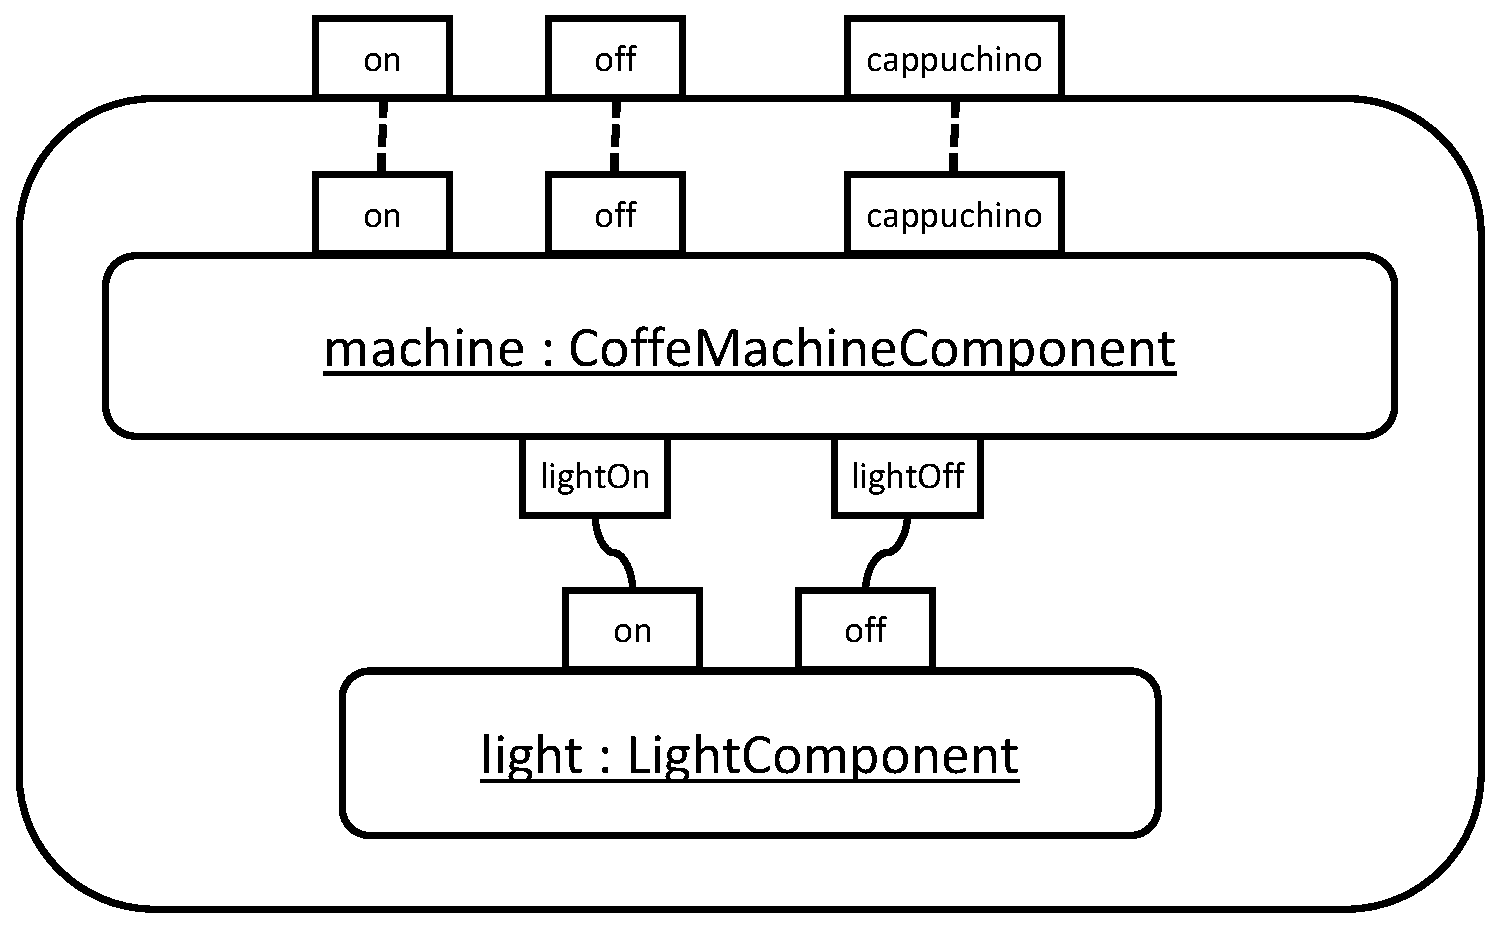
\includegraphics[width=0.455\textwidth]{figures/block_diagram_cropped2.pdf}%
	\caption{A composite system of a CoffeMachine and a LightSwitch statechart.}
	\label{fig:block_diagram_cropped2}
\end{figure}

Note that a composite system description constists of the following parts:

\begin{itemize}
	\item System interface definition: All input \textsl{Ports} of \emph{machine} are published to the interface of the system enabling the users to turn \emph{machine} on and off or order a cappuchino.
	
	\item Component interface definitions: \emph{CoffeMachineComponent} refers to \emph{on}, \emph{off} and \emph{cappuchino} through input \textsl{Ports} (denoted by the IN keyword) and \emph{flashLight}, \emph{turnOffLight} through output \textsl{Ports} (denoted by the OUT keyword). Both signal declarations of LightSwitch are referred to by input \textsl{Ports}.
	
	\item Component instantiations: Both \textsl{Components} are instantiated: \emph{machine} and \emph{light}.
	
	\item Channel definitions: The output \textsl{Ports} of \emph{machine} are connected to the input \textsl{Ports} of \emph{light}, making it possible for \emph{machine} to turn on \emph{light} at choice.
\end{itemize}

Figure \ref{fig:block_diagram_cropped2} depicts the composite system described by the previous code section.  Note that the individual components of the system are encapsulated. Interactions can be specified only through the defined interface.

\subsection{Semantics}
\label{sec:semantics}
 During the design of the semantics one of our goal was to define a language that enables the reuse of the source code generator of \Yakindu. Therefore the semantics of supported \Yakindu\ statecharts elements had to be considered, most importantly event raising.

This section introduces the semantics of the compositional language.
The compositional language enables to create a \emph{composite system}, that is formally a 4-tuple: $C = \langle\mathit{SC}, \mathit{CA}, \mathit{IN}, \mathit{OUT}\rangle$ where:

\begin{itemize}
	\item $\mathit{SC} = \{\langle S_1, s_1^0, T_1, I_1, O_1\rangle, \cdots, \langle S_n, s_n^0, T_n, I_n, O_n\rangle\}$ is a finite set of state machines.
	
	\item $I = \bigsqcup_{j = 1}^{n}I_j$, i.e.~the union of all in events of state machine components
	
	\item $O = \bigsqcup_{j = 1}^{n}O_j$, i.e.~the union of all out events of state machine components
	
	\item $\mathit{CA} \subseteq 2^O \times 2^I$, i.e.~channel associations relate a finite set of outputs to a finite set of inputs
	
	\item $\mathit{IN} \subseteq I $, i.e.~the input interface is a subset of the union of the in events of state machine components
	
	\item $\mathit{OUT} \subseteq O $, i.e.~the output interface is a subset of the union of the out events of state machine components
\end{itemize}
%A composition has a $\varrho$ \emph{run}, where:
A sequence of steps $\varrho = (\tau_1, \tau_2, \cdots)$ is called a \emph{complete run} of $C$ if the following conditions hold.

\begin{itemize}	
	
	\item $\tau_j = (\underline{s}_j, i_j, \underline{s}'_j, \underline{o}_j)$ is a single step that consists of a state vector representing each state of each component before the step, a finite set of inputs, a state vector representing each state of each component after the step and a finite set of outputs generated by each state machine components, where for all $1 \le k \le n$ at least one of the following conditions holds:
	\begin{itemize}
		\item $(i_j \cap I_k, \underline{s}_j[k], \underline{s}_j'[k], \underline{o}_j[k]) \in T_k$, i.e.~if a transition is defined in a state machine component that is triggered by the input set, then the transition fires taking the state machine to its target state and producing the corresponding outputs;		
		
		\item $ (\underline{s}_j[k] = \underline{s}_j'[k] \land \underline{o}_j[k] = \emptyset \land \nexists s', o':(i_j \cap I_k, \underline{s}_j[k], s', o') \in T_j)$, i.e.~a component is allowed to do nothing if and only if it has no transition that is triggered by input $i_j$ in state $\underline{s}_j[k]$;
	\end{itemize}	
	
	\item $\underline{s}_1 = (s_1^0, s_2^0, \cdots, s_n^0,)$, i.e.~at the beginning of the run, all state machine components are in their initial states;
	
	\item $\underline{s}_j'= \underline{s}_{j + 1}$, i.e.~the state vector at the end of a step and at the beginning of the next step are equal;
	
	\item $\mathit{tgd}(\bigcup_{k=1}^n \underline{o}_j[k]) \subseteq i_{j + 1} \subseteq \mathit{tgd}(\bigcup_{k=1}^n \underline{o}_j[k]) \cup \mathit{IN}$ where $\mathit{tgd}(\Omega) = \bigcup_{\omega \in 2^\Omega} \omega \circ \mathit{CA}$, i.e.~the inputs of a step is at least the inputs triggered through a channel by outputs of the previous step and maybe some additional events of the input interface;
	
	\item $\varrho$ is either infinite or the following condition holds:
	\begin{itemize}
		\item $\nexists (o,i) \in \mathit{CA}\colon o \cap o_n \neq \emptyset$, i.e.~the execution of steps can terminate only if the last step does not produce any outputs that will be inputs in the next step.
	\end{itemize}		
	
\end{itemize}	

A partial run of a composite system can be any prefix of a complete run (any other sequence is not considered to be a behavior of the composite system).

It is important to note that message queues (buffering) are not included, the semantics guarantees only that event raising and event receptions are in a causal relationship. Therefore, if a component does not buffer events (such as \Yakindu), parameterized events may overwrite each other.

The operational semantics presented above provides a way to reduce the semantics of the composite system to the semantics of the components. To formally analyze the system, denotational semantics has to be provided, e.g.~by model transformations converting the composite system model into a formal model, in accordance with the operational semantics.

%The compositional tool has a port system that differs from most tools of this field. Each \textsl{Port} of each \textsl{Instance} contains two \emph{cells}, an outer and an inner cell. A cell is a container for a signal. Whenever a signal arrives at one of the \textsl{Ports}, it is placed into the outer cell. If more than one signal arrives at the same \textsl{Port} in the same turn, only the last one is stored removing the former signal. This can be relevant when the particular \textsl{Port} refers to a signal declaration with a type. Otherwise, all the signals are identical. If the user wants to eliminate this possibility, we advise them to connect only one output \textsl{Port} to a particular input \textsl{Port}.

%The compositional tool adopts a turn-based semantic. At the beginning of each turn, the values of the outer cells are copied into the inner cells and the outer cells are emptied. After that, a scheduling turn begins. An \textsl{Instance} only takes notice of signals in the inner \textsl{Port} cells. The \textsl{Instances} are scheduled one after another. Although, the order of the scheduling is not defined, it is fixed, therefore they are scheduled in the same order in each turn. This does not cause a loss of generality, because the \textsl{Instances} can not affect each other in one scheduling turn, as an incoming signal is placed into the outer cell.

\section{Conclusions and Future Work}
\label{sec:conclusion}

\Yakindu\ is a popular open-source tool for the design of statechart models with support for code generation. It has a rich language to model a single hierarchical statechart, but it lacks the ability to compose statecharts into a component-based model. For the design of complex, embedded reactive systems, compositionality is essential to handle the design complexity. Moreover, a precise formal semantics is necessary to facilitate code generation and formal analysis.

The defined compositional language enables to instantiate \Yakindu\ statecharts, specify ports for these instances and join these instances through port connections. The semantics of the language is well-defined and suits the statechart semantics of \Yakindu\ soundly.

%Furthermore, we defined validation rules for the static analysis of both the statecharts and the composite systems. These rules provide the users with lots of information on their models at an early stage of design and restrict the features of \Yakindu\ to enable precise formalization.

Subject to future work, we plan to extend the compositional language to allow hierarchical compositions, i.e.~the composition of composite systems. Additionally, we intend to design a whole framework around the language that \textit{1)} enables the generation of source code which connects the \Yakindu\ statecharts according to the defined semantics and \textit{2)} provides automated model transformation to formal models of composite systems on which exhaustive analysis can be performed by model-checkers.

The automatic model transformers will utilize a graph-pattern-based approach to generate the traceability information that will facilitate the back-annotation of the results of formal analysis to the engineering domain. This way, we hope to support formal verification without requiring the designers to get familiar with the formal languages involved.

% An example of a floating figure using the graphicx package.
% Note that \label must occur AFTER (or within) \caption.
% For figures, \caption should occur after the \includegraphics.
% Note that IEEEtran v1.7 and later has special internal code that
% is designed to preserve the operation of \label within \caption
% even when the captionsoff option is in effect. However, because
% of issues like this, it may be the safest practice to put all your
% \label just after \caption rather than within \caption{}.
%
% Reminder: the "draftcls" or "draftclsnofoot", not "draft", class
% option should be used if it is desired that the figures are to be
% displayed while in draft mode.
%
%\begin{figure}[!t]
%\centering
%\includegraphics[width=2.5in]{myfigure}
% where an .eps filename suffix will be assumed under latex, 
% and a .pdf suffix will be assumed for pdflatex; or what has been declared
% via \DeclareGraphicsExtensions.
%\caption{Simulation results for the network.}
%\label{fig_sim}
%\end{figure}

% Note that the IEEE typically puts floats only at the top, even when this
% results in a large percentage of a column being occupied by floats.


% An example of a double column floating figure using two subfigures.
% (The subfig.sty package must be loaded for this to work.)
% The subfigure \label commands are set within each subfloat command,
% and the \label for the overall figure must come after \caption.
% \hfil is used as a separator to get equal spacing.
% Watch out that the combined width of all the subfigures on a 
% line do not exceed the text width or a line break will occur.
%
%\begin{figure*}[!t]
%\centering
%\subfloat[Case I]{\includegraphics[width=2.5in]{box}%
%\label{fig_first_case}}
%\hfil
%\subfloat[Case II]{\includegraphics[width=2.5in]{box}%
%\label{fig_second_case}}
%\caption{Simulation results for the network.}
%\label{fig_sim}
%\end{figure*}
%
% Note that often IEEE papers with subfigures do not employ subfigure
% captions (using the optional argument to \subfloat[]), but instead will
% reference/describe all of them (a), (b), etc., within the main caption.
% Be aware that for subfig.sty to generate the (a), (b), etc., subfigure
% labels, the optional argument to \subfloat must be present. If a
% subcaption is not desired, just leave its contents blank,
% e.g., \subfloat[].


% An example of a floating table. Note that, for IEEE style tables, the
% \caption command should come BEFORE the table and, given that table
% captions serve much like titles, are usually capitalized except for words
% such as a, an, and, as, at, but, by, for, in, nor, of, on, or, the, to
% and up, which are usually not capitalized unless they are the first or
% last word of the caption. Table text will default to \footnotesize as
% the IEEE normally uses this smaller font for tables.
% The \label must come after \caption as always.
%
%\begin{table}[!t]
%% increase table row spacing, adjust to taste
%\renewcommand{\arraystretch}{1.3}
% if using array.sty, it might be a good idea to tweak the value of
% \extrarowheight as needed to properly center the text within the cells
%\caption{An Example of a Table}
%\label{table_example}
%\centering
%% Some packages, such as MDW tools, offer better commands for making tables
%% than the plain LaTeX2e tabular which is used here.
%\begin{tabular}{|c||c|}
%\hline
%One & Two\\
%\hline
%Three & Four\\
%\hline
%\end{tabular}
%\end{table}


% Note that the IEEE does not put floats in the very first column
% - or typically anywhere on the first page for that matter. Also,
% in-text middle ("here") positioning is typically not used, but it
% is allowed and encouraged for Computer Society conferences (but
% not Computer Society journals). Most IEEE journals/conferences use
% top floats exclusively. 
% Note that, LaTeX2e, unlike IEEE journals/conferences, places
% footnotes above bottom floats. This can be corrected via the
% \fnbelowfloat command of the stfloats package.




% conference papers do not normally have an appendix


% use section* for acknowledgment
\section*{Acknowledgment}
This work was partially supported by IncQuery Labs Ltd. and MTA-BME Lend\"ulet Research Group on Cyber-Physical Systems.





% trigger a \newpage just before the given reference
% number - used to balance the columns on the last page
% adjust value as needed - may need to be readjusted if
% the document is modified later
%\IEEEtriggeratref{8}
% The "triggered" command can be changed if desired:
%\IEEEtriggercmd{\enlargethispage{-5in}}

% references section

% can use a bibliography generated by BibTeX as a .bbl file
% BibTeX documentation can be easily obtained at:
% http://mirror.ctan.org/biblio/bibtex/contrib/doc/
% The IEEEtran BibTeX style support page is at:
% http://www.michaelshell.org/tex/ieeetran/bibtex/
%\bibliographystyle{IEEEtran}
% argument is your BibTeX string definitions and bibliography database(s)
%\bibliography{IEEEabrv,../bib/paper}
%
% <OR> manually copy in the resultant .bbl file
% set second argument of \begin to the number of references
% (used to reserve space for the reference number labels box)
\bibliographystyle{IEEEtran}
\bibliography{IEEEabrv,./bib}






% that's all folks
\end{document}


